\tocless\subsection{Objective}
For this experiment, it was decided to take inspiration from
\parencite{yanaiFood}, where pre-training was used training a model for food
classification. In order to achieve this, the final layer of the
Inception V3 model which was trained on the ImageNet dataset had to be retrained. This is called
Transfer Learning.
A tutorial, created by Google, on the TensorFlow website was followed
for direction on this process \parencite{retrainInception}.

Firstly, to retrain the final layer of a model, a dataset must be
prepared in the correct way. The Food-101 dataset \parencite{food101}
was used for this experiment, which will be analysed below.

This dataset contrasts with \parencite{yanaiFood} as they used the UECFOOD100 dataset.
The food-101 dataset was chosen due to larger number of images per class.
The UECFOOD100 dataset has 100 images per class while the food-101 dataset has 1,000 images per class.
The dataset must be structured so that
there is a separated directory for each class with the directory name as the class
name. These directories should contain all the images for this class. 

Once this dataset has been set up correctly, a directory can be found on GitHub
which contains the necessary files for this tutorial. When the directory has
been downloaded, the following command can be executed:
\begin{figure}
\caption{Retrain Inception Command}
\label{lst:retrainCommand}
\begin{lstlisting}[style=Command]
python tensorflow/examples/image_retraining/retrain.py \ --image_dir
~/dataset_directory
\end{lstlisting}
\end{figure}

The first thing that the script will do is create bottleneck files for the
images. A bottleneck is a term used to define the final layer before the output
layer. This is so that for each image, we do not have to push it through the
entire network during training \parencite{retrainInception}.

After, the bottlenecks are created, the training can be completed. The images
are split into three sub directories of training, testing and validation. By
default, these images are split into percentages of 80\%, 10\% and 10\%
respectively. The model is trained at a default of 4,000 steps. 

At the final stage of the script, the model is run on a batch of test images not
yet seen and a final test accuracy is displayed. This can be seen in the Script
section below.

The command used for using this model once it is trained is:
\begin{figure}
\caption{Label Image Command}
\label{lst:labelImage}
\begin{lstlisting}[style=Command]
python tensorflow/examples/label_image.py --graph=/tmp/output_graph.pb
--labels=/tmp/output_labels.txt --input_layer=Mul --output_layer=final_result
--input_mean=128 --input_std=128 --image=~/image_directory
\end{lstlisting}
\end{figure}

\begin{table}[h]
\centering
\caption{Retrain ImageNet Inception V3 Model}
\label{my-label}
\begin{tabular}{|l|p{8cm}|}
\hline
\textbf{Network Architecture} & Inception-V3 architecture \parencite{inception}            \\ \hline
\textbf{Dataset}              & Food-101 dataset \\ \hline
\textbf{APIs and Libraries}   & TensorFlow and NumPy                                                        \\ \hline
\end{tabular}
\end{table}

\tocless\subsection{Script}
The following snippets of code in Figure \ref{lst:addNewLayer} and Figure \ref{lst:evalModel} are from the retrain.py script.
Figure \ref{lst:addNewLayer} defines howto add a new layer to the top of the network while Figure \ref{lst:evalModel} defines how to evaluate the accuracy of the new layer. 

\begin{figure}
\caption{Add New Layer \parencite{retrainInception}}
\label{lst:addNewLayer}
\begin{lstlisting}[style=Python]
# Add new layer to the network
(train_step, cross_entropy, bottleneck_input, ground_truth_input,
final_tensor) = add_final_training_ops(
            len(image_lists.keys()), FLAGS.final_tensor_name,
            bottleneck_tensor,
            model_info['bottleneck_tensor_size'],
            model_info['quantize_layer'])
 
# Create operations to evaluate the accuracy of the model
evaluation_step, prediction = add_evaluation_step(
final_tensor, ground_truth_input)
 
# Set up weights to initial default values.
init = tf.global_variables_initializer()
sess.run(init)
\end{lstlisting}
\end{figure}

\begin{figure}
\caption{Evaluate Model \parencite{retrainInception}}
\label{lst:evalModel}
\begin{lstlisting}[style=Python]
# Run final test evaluation
test_bottlenecks, test_ground_truth, test_filenames = (
    get_random_cached_bottlenecks(
        sess, image_lists, FLAGS.test_batch_size, 'testing',
        FLAGS.bottleneck_dir, FLAGS.image_dir, jpeg_data_tensor,
        decoded_image_tensor, resized_image_tensor, bottleneck_tensor,
        FLAGS.architecture))
test_accuracy, predictions = sess.run(
   [evaluation_step, prediction],
   feed_dict={bottleneck_input: test_bottlenecks,
        ground_truth_input: test_ground_truth})
tf.logging.info('Final test accuracy = %.1f%% (N=%d)' %
                (test_accuracy * 100, len(test_bottlenecks)))
\end{lstlisting}
\end{figure}

\tocless\subsection{Results}
The final test Top-1 accuracy for this retrained model was 54.8\%.
These results are calculated by passing an unseen batch of test images through the model.
The 95\% confidence interval of the Top-1 accuracy of this model is between 45.1\% and 64.5\%.
This confidence interval was calculated by Equation \ref{eqn:ci}.

\begin{equation}\label{eqn:ci}
    e \pm 1.96\sqrt{e(1-e) \over n}
\end{equation}

An image of pizza Figure \ref{fig:pizza}, was fed into the model with the following results:
\begin{itemize}
    \item{pizza 0.925}
    \item{pancakes 0.008}
    \item{nachos 0.007}
    \item{beef carpaccio 0.006}
    \item{tiramisu 0.004}
\end{itemize}
In contrast, Figure \ref{fig:pizza_unclassified} was not classified as a pizza.

\begin{figure}[h] 
\centering
  \label{pizzas} 
  \begin{minipage}[h]{0.5\linewidth}
    \centering
    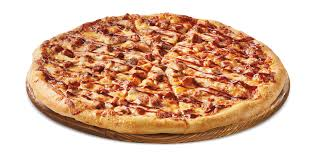
\includegraphics[scale=0.5]{pizza} 
    \caption{Pizza - sourced from https://www.cicis.com/} 
  \label{fig:pizza}
    \vspace{4ex}
  \end{minipage}%%
  \begin{minipage}[h]{0.5\linewidth}
    \centering
    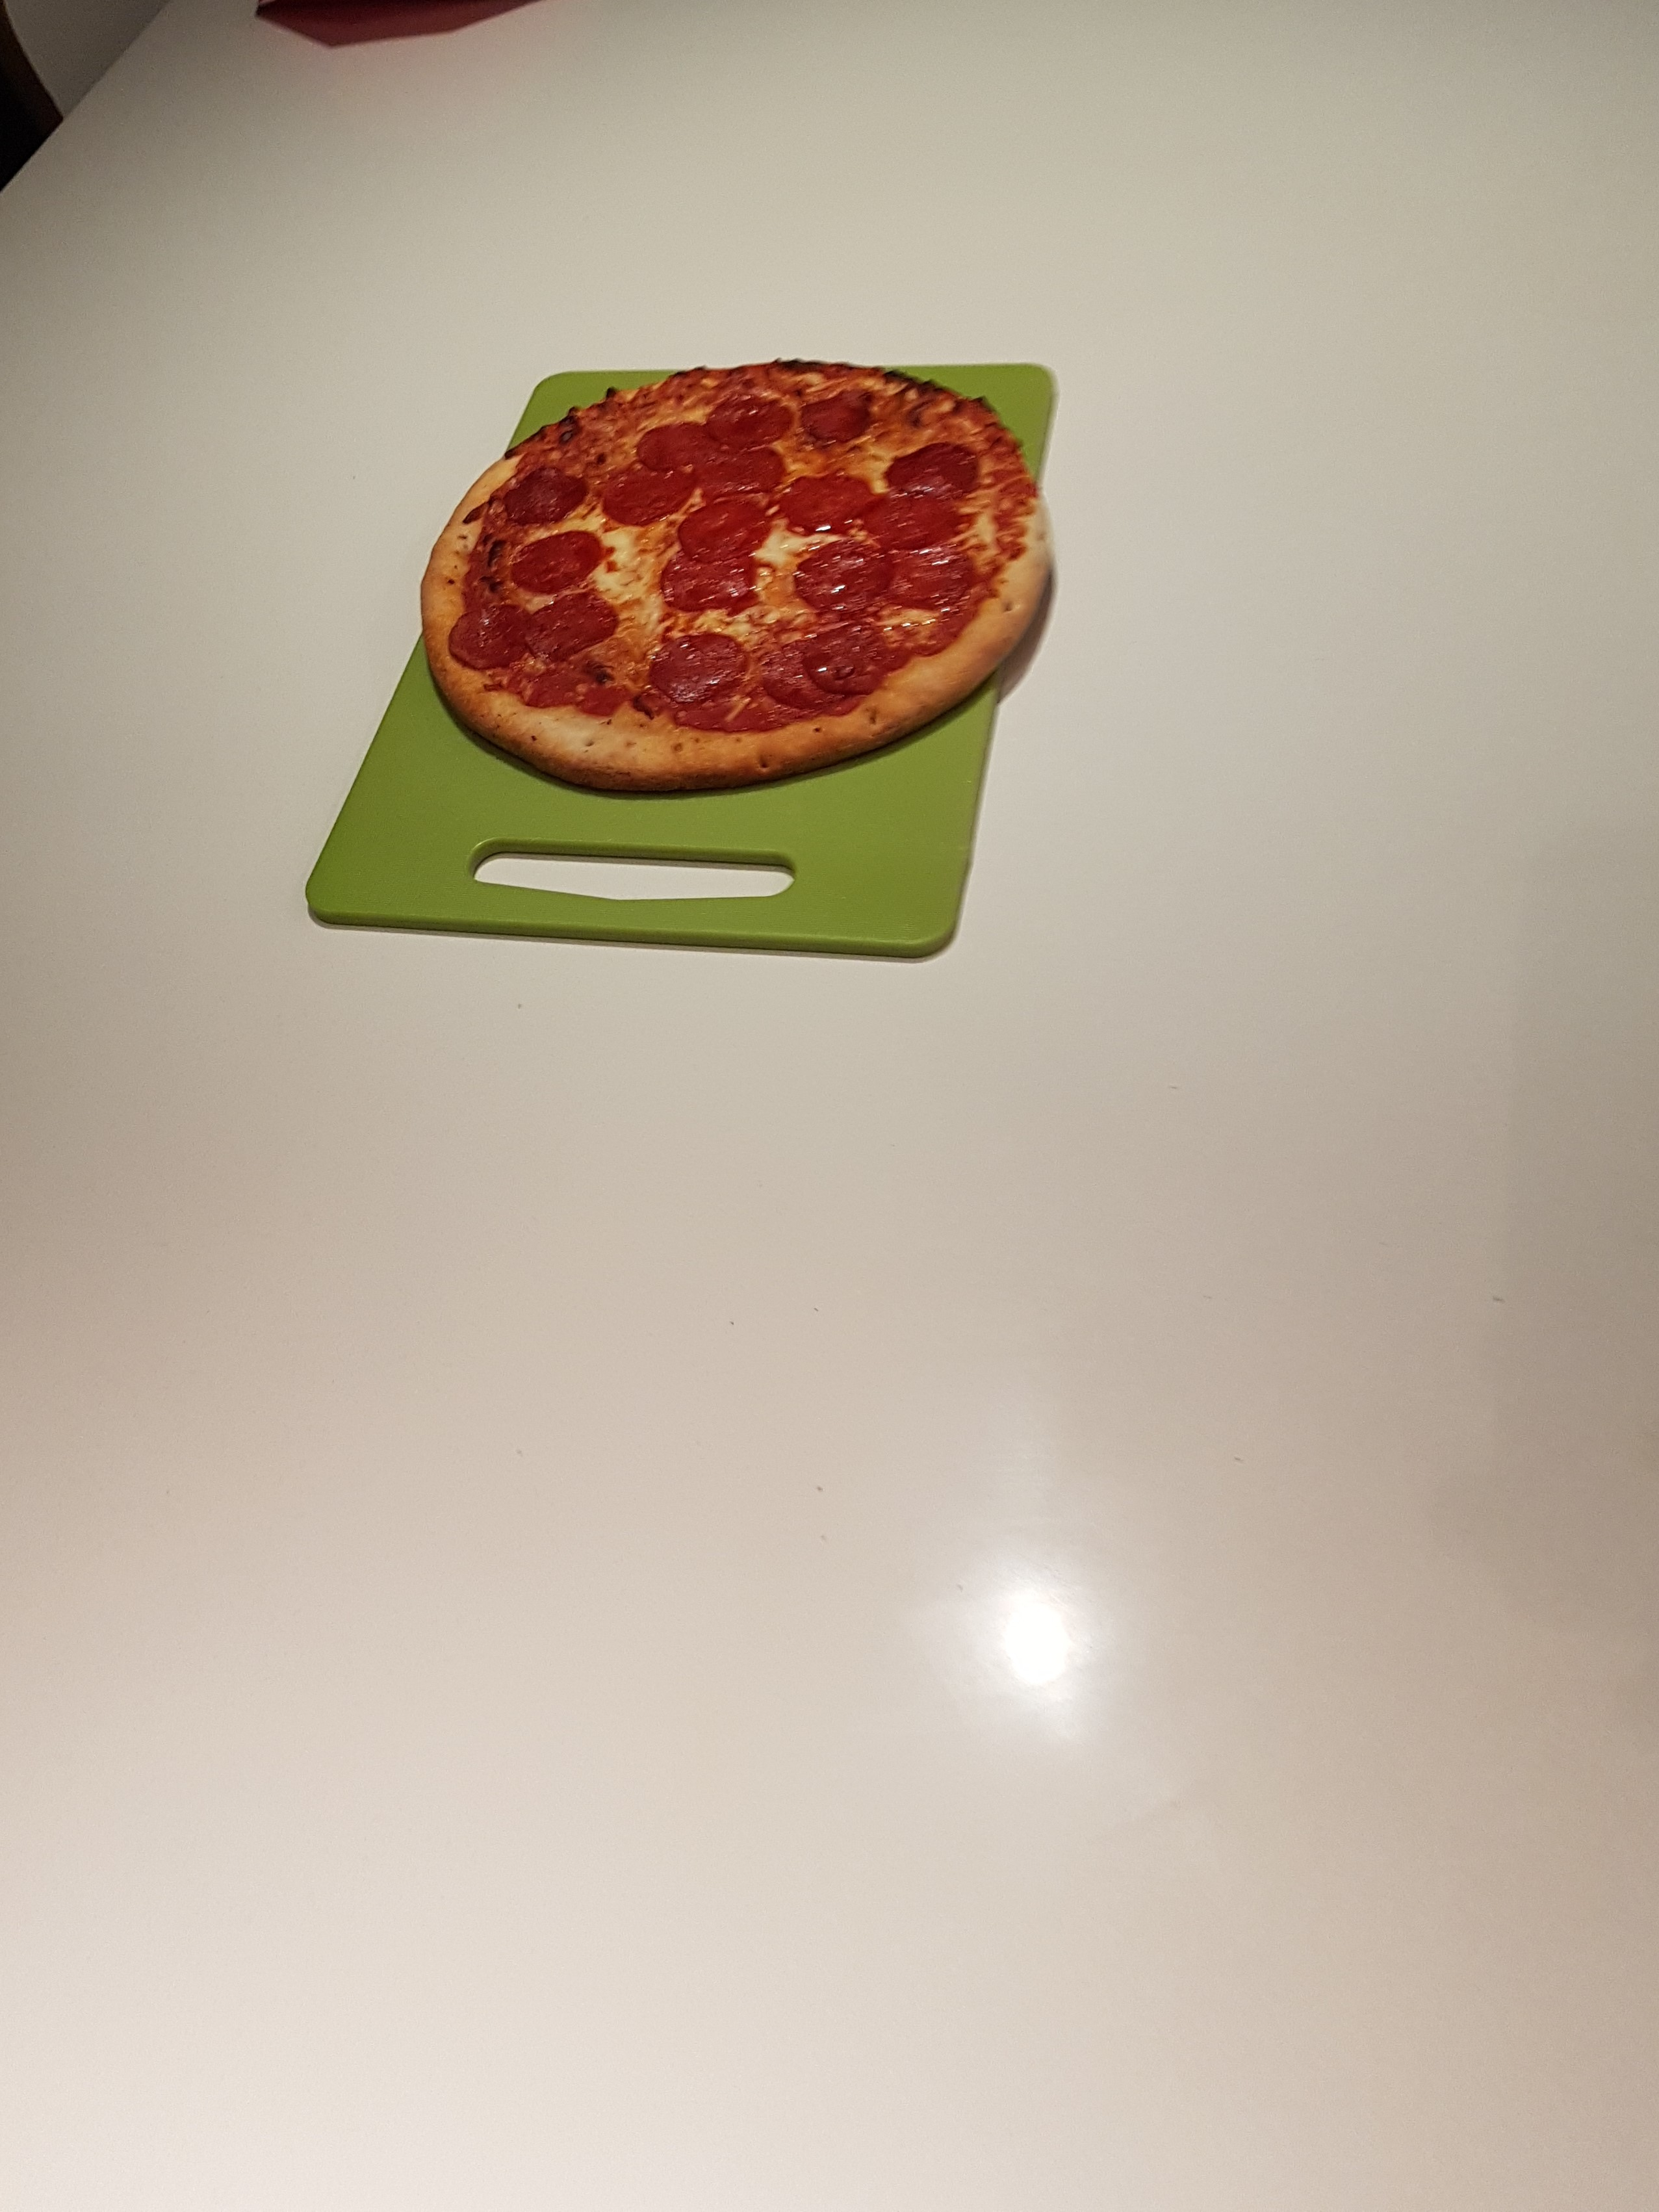
\includegraphics[scale=0.065]{pizza_unclassified} 
    \caption{Pizza not classified correctly by the model} 
  \label{fig:pizza_unclassified}
    \vspace{4ex}
  \end{minipage} 
\end{figure}

\tocless\subsection{Analysis}
These poor results are not that surprising.
This is because we have many classes to train for, 101, and no parameter tuning has been carried out on the running of this code.
Figure \ref{fig:pizza_unclassified} was not classified correctly, this is most likely due to the fact that the pizza does not take up much of the image.

\afterpage{\clearpage}